% !TEX encoding = UTF-8 Unicode
%!TEX root = ../Main/thesis.tex
% !TEX spellcheck = en-US
%%=========================================
\documentclass[../Main/thesis.tex]{subfiles}
\begin{document}
\chapter{First Iteration  - Establishing requirements}
\label{ch:requirements}
This chapter describes the first step in the development process: establishing requirements for the system. 

\section{Initial requirements}
The first requirements that were established was the overall structure of the system and which technologies should be used.
It was decided that BLE should be used as the technology for localization.
The data from the BLE beacons should be collected using cellphones, running the Android operation system, attached to the smoke divers.
This data should then be visualized in a web interface.

The initial requirements was then:
An Android application that could track the Bluetooth signal from the beacons and upload them to a server.
A back-end that could receive data from the cellphone, process the raw data and present it through a REST API.
A web-application for presenting and visualizing the processed data from the back-end.

\subsection{Android Application}
Before the initial meeting with Øygarden Fire and Rescue (ØFR) a design-prototype of the Android application was created. 
This purpose of this prototype was to showcase both a suggestion of how the application would be used, and, most important, how the app should function.
The first step in creating the prototype was to create the flowchart shown in Figure~\ref{fig:flow-app-1}, visualizing user actions in the app.

\begin{figure}
	\centering
	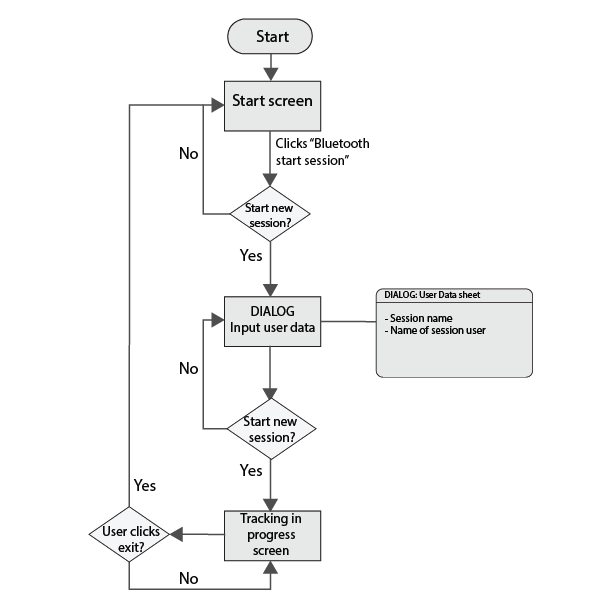
\includegraphics[width=0.6\linewidth]{../fig/flow_wire_app_1}
	\caption{Flowchart of the Android application}
	\label{fig:flow-app-1}
\end{figure}

As the application only have one feature, it should be as simple as possible. 
The user of the application should be able to create a new session with a name and a user and start the session. 
Then the application should collect data from nearby BLE devices until the user end the session.
The application should then upload the collected data to the server for processing.

When the initial requirements was included in the flowchart a wireframe was created as shown in Figure~\ref{fig:wireframe-app-1}.
This was created both to present a possible design, and to present how the app could be used to the firefighters. 

\begin{figure}
	\centering
	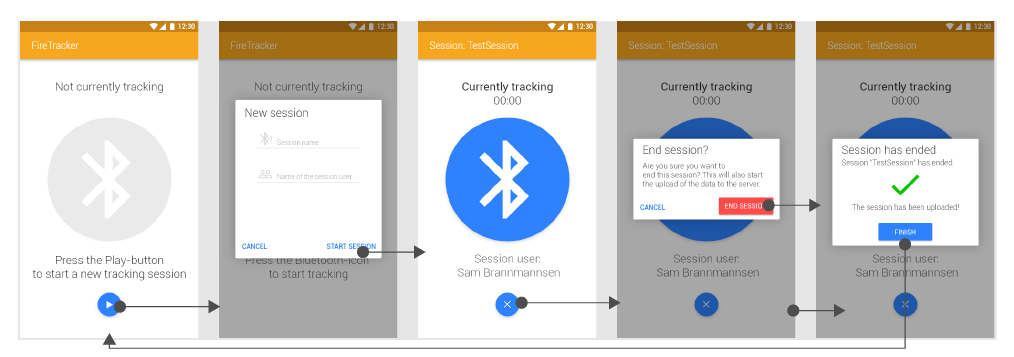
\includegraphics[width=\linewidth]{../fig/wireframe_app_1}
	\caption{Wireframe of the Android application}
	\label{fig:wireframe-app-1}
\end{figure}

\subsection{Back-end}
At this stage the only defined requirements for the back-end was that it should be able to receive data through a REST API, process the data, and present it through a REST API.

\section{Input from the fire department}
The requirements established this far was based on previous experience with development and an idea of how this system could be used, and what the fire department needed.
To better understand what they actually need, and how they think they can use the system, an interview with the fire chief and one of the instructors was conducted.
The interview session started with an observation of a smoke diving exercise and was then followed by the actual interview, which can be divided into three main parts: practical aspects, visualization and presentation of data, and use of data.
The interview was 20 minutes long, and it was recorded an transcribed.
The Norwegian interview-guide is attached in Appendix~\ref{app:interview-guide-first}.


\subsection{Practical questions}
In this section the fire chief and instructor were asked about practical aspects of the exercise and use of the system.
The following questions were asked:
\begin{itemize}
	\item How do you prepare for the exercise?
	\item Where can the cellphone be placed on the smoke diver?
	\item How many smoke divers participate in an exercise?
\end{itemize}

\subsubsection*{Summary of answers:}
\textit{Question 1:} 
The smoke divers know there is going to be an exercise, but not where or how it is going to be, and they try to vary the locations to prevent the smoke divers from ``getting used'' to a location or building.
ØFR has three teams of firefighters operating out of different fire stations so they also try to get locations that can be used for four weeks to use it for all three teams.
The instructors are able to prepare the location before the exercise and can then place beacons in the building.

\textit{Question 2:} 
As Bluetooth signals are easily blocked or reduced by the body it could be useful to place the receiver as high as possible on the smoke diver. **Find reference**
The device could be attached to the helmet or on top of the oxygen-tank.

\textit{Question 3:} 
The number of participants vary.
At this exercise they were 7 or 8, but if they exercise with firefighters from all three stations they could be 12.
In the building itself there are usually one team consisting of two smoke divers inside and one outside.
The one on the outside is responsible for communicating with those who are inside, and if something happens and they need assistance he can go in to help them get out.

\subsection{Visualization questions}
\begin{enumerate}
	\item What information can this kind of data give?
	\item How should the data be presented?
\end{enumerate}

\subsubsection*{Summary of answers:}
\textit{Question 1:}
It would be useful information about their search-technique, and search-coverage as one could see if there are areas or rooms that was not covered in the search.
If there is a room that was not searched this information could be used to discuss why this happened.
The data can be used as a reminder of events for the smoke divers in their evaluation after the exercise.

\textit{Question 2:}
A visualization of the data on top of a map or drawing of the floor plan for the building would be useful.
A list of visited locations with information about the time spent there would also be useful.

\subsection{Questions about using the data}
\begin{enumerate}
	\item Could this system have any negative consequences for the training, evaluation or feedback?
	\begin{itemize}
		\item Could it make the firefighters focus on the fact that they are being tracked instead of their tasks?
	\end{itemize}
	\item Could this system give the firefighters better feedback after the exercise?
	\item Could this system be used in further training of the firefighters?
	\begin{itemize}
		\item If yes: How?
	\end{itemize}
\end{enumerate}

\subsubsection*{Summary of answers:}
\textit{Question 1:}
The system should not affect the firefighters in any particular way.
They are so focused on their tasks, and they do not have time to think about other elements such as this system.
If anything it could lead to them putting extra effort into perfecting the tasks that are in focus in this exercise.

\textit{Question 2:}
As both the instructor and the firefighter would be able to actually see how they searched the building they could get a more detailed feedback with more information to reflect upon.

\textit{Question 3:}
It could be useful for the other firefighters, who did not perform a smoke dive in this exercise because they had another role, to see how the smoke divers performed, and to learn from their experiences and feedback.

\subsection{Analysis of interview}
They are clearly interested in a system such as FireTracker, as it could improve the evaluation of an exercise, and the individual feedback to each smoke diver.
For their search-technique training, which is a major part of the smoke diving training, it would be useful to see which rooms or areas the smoke divers have visited and which they have not visited, together with the route they took through the area.
As they change locations for their training fairly often a mobile system that is easy to set up and move is needed.

\end{document}
